\documentclass[journal]{IEEEtran}

\usepackage{amsmath,amssymb,amsthm}
\usepackage{graphicx}
\usepackage{booktabs}
\usepackage{url}
\usepackage{algorithm}
\usepackage[noend]{algpseudocode}
\usepackage{cite}
\usepackage{multirow}
\usepackage{tikz}
\usetikzlibrary{positioning,arrows.meta,shapes.geometric}
\usepackage{xcolor}

\newtheorem{theorem}{Theorem}
\newtheorem{corollary}{Corollary}
\newtheorem{definition}{Definition}

\begin{document}

\title{When Do Simple Formulas Beat Ensembles?\\
A 31-Dataset Benchmark for Interpretable\\Binary Classification}

% Double-anonymous: author info removed for review
\author{Anonymous}

\markboth{IEEE Transactions on Artificial Intelligence}
{Anonymous: Simple Formulas vs.\ Ensembles}

\maketitle

\begin{abstract}
When can a short algebraic formula replace a gradient-boosted
ensemble for binary classification on tabular data?  We answer this
question empirically on 31 UCI/OpenML datasets using a unified
protocol: each dataset is evaluated with $200 \times 5$-fold
repeated stratified cross-validation (1{,}000 paired measurements),
comparing depth-3 symbolic formulas against gradient boosting,
random forest, and logistic regression under identical train/test
splits.

The search engine---Theory Radar---searches a bounded depth-3
formula family via GPU beam search and random-subspace exploration
over 10 binary and 6 unary operators, evaluates each candidate with
exact $O(N \log N)$ sort-and-sweep $F_1$ optimization, and uses PLS
projections to give three-term formulas implicit access to all $d$
features.  A meta-learned pruning
technique discovers safe pruning rules from exhaustive micro-search,
eliminating 88--99.6\% of dead subtrees with zero false negatives
within the exhaustive micro-search space (extrapolation to deeper
search is empirical).  The benchmark results below use the unpruned
beam search; pruning is evaluated separately as a search-efficiency
contribution.

On 9 of 31 datasets (29\%), the formula beats default
gradient boosting: Liver ($\Delta F_1 = {+}0.159$), Haberman
($\Delta F_1 = {+}0.175$), Transfusion ($\Delta F_1 = {+}0.118$),
Vertebral ($\Delta F_1 = {+}0.060$), Diabetes
($\Delta F_1 = {+}0.032$), Wine ($\Delta F_1 = {+}0.035$), Heart
($\Delta F_1 = {+}0.028$), Hepatitis ($\Delta F_1 = {+}0.021$),
and Breast~Cancer ($\Delta F_1 = {+}0.006$).  Three datasets are
statistical ties, and 19 are ensemble wins.  Winning datasets share
a common profile: moderate sample size ($N \leq 800$), a
discriminative subspace captured by 2--3 PLS components, and
medical/clinical provenance.  We report all results honestly,
including the 19 losses, and provide PLS loading analyses showing
that winning formulas map to domain-interpretable feature
combinations.  Depth experiments to depth~9 with 5$\times$-wider
beams confirm that depth~3 provides the best generalization on
29 of 31 datasets.

Code: available upon acceptance (anonymous review).
\end{abstract}

% ================================================================
\section{Introduction}

A practitioner training a classifier on tabular data faces a
recurring question: \emph{do I need a 100-tree ensemble, or would a
simple formula suffice?}  If a formula works, it is auditable,
regulatable under the EU AI Act~\cite{euaiact2024} and FDA clinical
guidance~\cite{fda2022clinical}, and computable by hand.  If it does
not, the practitioner needs to know how much accuracy
interpretability costs on their specific data.

Few existing tools provide a systematic empirical comparison within a
defined formula class.  Genetic symbolic
regression~\cite{schmidt2009distilling,cranmer2023interpretable}
explores deep formula trees without fair evaluation protocols or
bounded search spaces.  Neural equation
discovery~\cite{udrescu2020ai} targets physics regression, not
classification.  Search-based
methods~\cite{kommenda2020search} enumerate small expressions but
optimize regression loss, not classification metrics.  Rule-based
interpretable models~\cite{breiman1984cart,letham2015interpretable,yang2017scalable}
produce discrete decision rules rather than continuous algebraic
formulas.  Post-hoc explainers such as
SHAP~\cite{lundberg2017unified} and LIME~\cite{ribeiro2016should}
explain a black box rather than replacing it.

This paper takes a direct approach: we build a tool---Theory
Radar---that searches a bounded depth-3 formula family using GPU beam search, evaluates
candidates under the same cross-validation protocol used for
baselines, and reports the outcome---win, tie, or loss---honestly
for every dataset.  The tool is designed around three principles:
(i)~\emph{bounded search} (the formula space is finite and
well-defined), (ii)~\emph{fair evaluation} (formulas and baselines
are scored on identical train/test splits with no methodological
asymmetry), and (iii)~\emph{honest reporting} (losses are reported
alongside wins, with effect sizes and confidence intervals for all
31 datasets).  We then analyze \emph{when} formulas win and
\emph{why}, grounding the analysis in PLS loading vectors that make
the formulas domain-interpretable.

Our contributions are:
\begin{enumerate}
\item A \textbf{31-dataset benchmark} with a unified evaluation
protocol ($200 \times 5$-fold CV, three baselines, effect-size
statistical reporting) that identifies 9 datasets where
depth-3 formulas beat default gradient boosting, 3 ties, and 19 losses.
\item A \textbf{characterization of the interpretability decision
boundary}: formulas win on moderate-$N$, medical/clinical
datasets whose discriminative subspace is low-dimensional.
\item A \textbf{meta-learned pruning} technique that discovers
safe pruning rules from exhaustive micro-search, pruning
88--99.6\% of dead subtrees with zero false negatives
\emph{within the enumerated depth-3 space} (application to
deeper search is an empirical extrapolation).
\item An \textbf{interpretability analysis} showing that PLS
loading vectors make winning formulas transparent:
clinically meaningful features (glucose, BMI, cell geometry)
dominate the projections.
\end{enumerate}

% ================================================================
\section{Related Work}
\label{sec:related}

\textbf{Genetic programming and symbolic regression.}
Symbolic regression originated with GP approaches that evolve
mathematical expressions to fit data~\cite{schmidt2009distilling}.
Schmidt and Lipson's landmark work demonstrated that free-form
equations could be distilled from experimental observations, but their
method optimizes mean squared error on regression targets and provides
no mechanism for classification.  Modern systems include
PySR~\cite{cranmer2023interpretable}, which uses multi-population
evolutionary search with regularized evolution and Pareto-optimal
complexity control.  PySR is arguably the current state of the art for
symbolic regression, but it explores deep expression trees without
bounding the search space and without fair cross-validated comparison
against ensemble classifiers on the same train/test splits.  Our
approach differs in three key respects: (i)~we bound the formula space
to depth~3 via beam search and random-subspace exploration; (ii)~we optimize $F_1$
directly via sort-and-sweep rather than regression loss; and (iii)~we
evaluate under the same $200 \times 5$-fold protocol used for all
baselines, ensuring methodological symmetry.

\textbf{Rule-based interpretable models.}
CART decision trees~\cite{breiman1984cart} produce axis-aligned
splits that are interpretable but greedy, unstable under small data
perturbations, and structurally limited to rectangular decision
regions.  Bayesian rule lists~\cite{letham2015interpretable} learn
ordered if-then rules with Bayesian priors on rule length, producing
more stable models with principled complexity control; however, the
rules are discrete (thresholded feature comparisons) and cannot
express continuous algebraic relationships.  Scalable Bayesian rule
lists~\cite{yang2017scalable} extend this framework to larger
datasets via parallelized posterior sampling.  These models are
inherently discrete (rules over feature thresholds), whereas our
method discovers continuous algebraic formulas that can capture
smooth decision boundaries---the two approaches are complementary.
A rule list partitions the feature space into disjoint regions; a
symbolic formula defines a continuous score function thresholded
once.  On datasets where the boundary is smooth (e.g., Diabetes,
where glucose and BMI interact continuously), algebraic formulas have
a structural advantage.

\textbf{Post-hoc explainability.}
SHAP~\cite{lundberg2017unified} assigns Shapley-value attributions
to input features, decomposing each prediction into additive
contributions.  LIME~\cite{ribeiro2016should} fits local linear
surrogates around individual predictions.  Both methods have become
standard tools for model auditing, but they share a fundamental
limitation: they explain \emph{what} a black-box model does on a
given input, not \emph{whether a simpler model would perform equally
well globally}.  A SHAP analysis of a gradient-boosted classifier
tells a clinician which features drove a specific prediction; it does
not tell the clinician whether a three-term formula would have
produced the same accuracy across all patients.  Our approach answers
this replacement question directly: rather than explaining the
ensemble, we attempt to replace it and report the outcome.

\textbf{Neural equation discovery.}
AI Feynman~\cite{udrescu2020ai} discovers physical equations using
neural networks to identify symmetries (translational, rotational,
separability), then applies symbolic regression in the simplified
subspaces.  It targets physics problems: continuous, low-noise data
with exact underlying equations, and optimizes regression loss
(MSE).  The classification setting differs fundamentally: targets are
binary, noise is high, and the relevant metric is $F_1$ (which
balances precision and recall on the minority class) rather than
reconstruction error.  Our method is designed for this setting:
sort-and-sweep $F_1$ optimization, PLS projections for
discriminative subspaces, and systematic comparison against ensemble
baselines on tabular data.

\textbf{Search-based symbolic regression.}
Kommenda et al.~\cite{kommenda2020search} enumerate small expressions
and fit parameters via nonlinear least squares, achieving strong
regression accuracy on benchmark problems.  Their enumeration
strategy shares our philosophy of bounded search, but the focus is
regression accuracy with parameter fitting rather than classification
with threshold optimization.  Our sort-and-sweep $F_1$ evaluation is
parameter-free (the threshold is found exactly in $O(N \log N)$),
and our meta-learned pruning discovers safe subtree elimination rules
that their framework does not address.

\textbf{Positioning.}
Theory Radar occupies a distinct niche in this landscape: it is
a system that performs bounded symbolic search
with direct $F_1$ optimization, fair cross-validated comparison
against ensemble baselines, and honest reporting of both wins and
losses across a large dataset collection.  Existing approaches either
optimize the wrong metric (regression loss), use unbounded search
(GP/PySR), produce discrete rules rather than continuous formulas
(Bayesian rule lists), or explain rather than replace the black box
(SHAP/LIME).

% ================================================================
\section{Method}
\label{sec:method}

\subsection{Core Engine}
\label{sec:core}

The search generates candidate formula trees to depth $D = 3$ over a
set of binary operators $\mathcal{B}$ and unary operators
$\mathcal{U}$.  Each candidate maps input features
$\mathbf{x} \in \mathbb{R}^d$ to a scalar score $f(\mathbf{x})$.
The classifier is
$\hat{y} = \mathbf{1}[f(\mathbf{x}) > \tau]$ \emph{or}
$\hat{y} = \mathbf{1}[f(\mathbf{x}) < \tau]$, with the threshold
$\tau$ and direction chosen to maximize $F_1$ on training data.
Both directions are always evaluated.

\textbf{Sort-and-sweep $F_1$.}
For a candidate producing scores $\{f(\mathbf{x}_i)\}_{i=1}^N$,
the optimal threshold is found by sorting scores, then sweeping
through threshold positions while maintaining running counts of
true positives (TP), false positives (FP), and false negatives (FN).
Concretely, let $\pi$ be the permutation that sorts scores in
ascending order.  Initialize the ``$>$'' direction with
$\mathrm{TP} = P$ (the total number of positives) and $\mathrm{FP} = N - P$.
Starting from the lowest score, move the threshold rightward one
sample at a time: if $y_{\pi(i)} = 1$, decrement TP; otherwise
decrement FP.  At each position, compute
$F_1 = 2\,\mathrm{TP} / (2\,\mathrm{TP} + \mathrm{FP} + \mathrm{FN})$
and record the maximum.  The ``$<$'' direction is evaluated
symmetrically by sweeping from the highest score downward.  The
overall optimal threshold and direction are the combination
achieving the highest $F_1$.

This procedure yields the \emph{exact} $\arg\max_\tau F_1$ in
$O(N \log N)$ time (dominated by the sort), with the sweep itself
being $O(N)$.  No grid search, no approximation---every possible
threshold position is evaluated.  This is critical for formula
search: candidates whose discrimination signal is concentrated in
a narrow score range (common for formulas involving $\log$ or
$\sigma$) would be missed by coarse threshold grids.

Constant-valued candidates (standard deviation $< 10^{-12}$) are
assigned $F_1 = 0$ to prevent sort-order artifacts from producing
spurious scores.  Candidates producing NaN or infinite values are
sanitized via \texttt{nan\_to\_num} before sorting.

\textbf{FormulaTrace and fair evaluation.}
Each formula's operation sequence is recorded in a
\texttt{FormulaTrace} object that stores the sequence of operators,
feature indices, and any PLS projection matrices used during
construction.  After search, the formula is replayed on held-out
test data by applying the \emph{same} sequence of operations with
the \emph{same} PLS projection matrix (fit on training data only),
thresholded using the cutoff tuned on training data, and scored on
the test split.  This replay mechanism is critical for fair
evaluation: it ensures that the formula's test-time behavior is
fully determined by training-time decisions, with no leakage of
test data into threshold selection or projection fitting.  This is
identical to how sklearn baselines are evaluated (fit on training
data, predict on test data, score on test predictions)---there is
no methodological asymmetry between the formula and any baseline.

\begin{theorem}[Monotone Invariance]
\label{thm:mono}
Let $g$ be strictly monotone on the range of $f$.  Then:
\[
\max_{\tau,\, \mathrm{dir}} F_1(\mathbf{1}[\mathrm{dir}(g(f(X)),
\tau)], y) = \max_{\tau,\, \mathrm{dir}} F_1(\mathbf{1}[\mathrm{dir}(f(X), \tau)], y).
\]
\end{theorem}

\begin{proof}
If $g$ is increasing, $g(f(x)) > \tau \Leftrightarrow f(x) >
g^{-1}(\tau)$.  If decreasing, $g(f(x)) > \tau \Leftrightarrow
f(x) < g^{-1}(\tau)$.  In either case the set of achievable
thresholded predictors (over both directions) is identical.
\end{proof}

\begin{corollary}[Monotone $F_1$ Reuse]
When expanding a node $f$ via a monotone unary operation $g$,
the child $g(f)$ has the same optimal $F_1$ as $f$.  The search
reuses the parent's $F_1$, saving one $O(N \log N)$ evaluation.
This does \emph{not} justify pruning the subtree rooted at
$g(f)$, since descendants like $(g(f))^2$ may differ from $f^2$.
\end{corollary}

\begin{corollary}[AUROC Invariance Under Monotone Transforms]
AUROC depends only on rank ordering.  An increasing $g$ preserves
rank order; a decreasing $g$ reverses it.  Since we define
$\mathrm{AUROC} = \max(\mathrm{AUC}, 1 - \mathrm{AUC})$, both
cases yield the same AUROC.
\end{corollary}

\subsection{Search Accelerators}
\label{sec:search}

\textbf{GPU-accelerated beam search.}
Given a beam of $B$ formulas $\mathbf{V} \in \mathbb{R}^{N \times B}$
and features $\mathbf{X} \in \mathbb{R}^{N \times d}$, each binary
operation $\circ \in \mathcal{B}$ produces $B \cdot d$ candidates via
tensor broadcasting:
$\mathbf{C}_\circ = \mathbf{V}_{(:,:,1)} \circ \mathbf{X}_{(:,1,:)}
\in \mathbb{R}^{N \times B \times d}$.
All candidates are stacked, sort-and-sweep $F_1$ is computed in a
single batched GPU call, and the top $B$ candidates are retained.

\textbf{Random-subspace fuzzing.}
To explore diverse feature combinations on high-dimensional datasets,
the search runs 15 independent subspace trials, each sampling
$\min(10, d)$ features uniformly at random.  The best formula across
all subspaces is reported.

\textbf{Meta-learned pruning.}
This is the primary algorithmic contribution: the search applied to
itself.  Given exhaustive enumeration of formulas to depth $D$, each
shallow node $n$ is classified as \emph{alive} (its subtree contains
a near-optimal formula) or \emph{dead} (safe to prune).  We then
search for a formula $\phi$ over node meta-features such that
$\phi(n) < \theta \implies n \text{ is dead}$, where
$\theta = \min_{n:\,\text{alive}} \phi(n)$, guaranteeing zero false
negatives by construction.

A family of 12 candidate criteria is evaluated.  Each criterion is a
simple algebraic function of four node meta-features: the node's
training $F_1$, its AUROC, its formula depth $k$, and the number of
features $d$ referenced.  The 12 criteria are:
\begin{enumerate}
\setlength{\itemsep}{0pt}
\item $F_1$ alone
\item $\text{AUROC}$ alone
\item $F_1 / k$
\item $F_1 / d$
\item $\text{AUROC} / k$
\item $\text{AUROC} / d$
\item $F_1 \cdot \text{AUROC}$
\item $F_1 \cdot \text{AUROC} / k$
\item $F_1 \cdot \text{AUROC} / d$
\item $F_1 + \text{AUROC}$
\item $(F_1 + \text{AUROC}) / k$
\item $(F_1 + \text{AUROC}) / d$
\end{enumerate}
For each criterion $\phi_j$, the threshold is set at
$\theta_j = \min_{n:\,\text{alive}} \phi_j(n)$, guaranteeing zero
false negatives by construction.  The prune rate is then
$|\{n : \phi_j(n) < \theta_j \land n\text{ is dead}\}| / |\{n : n\text{ is dead}\}|$.
The criterion with the highest prune rate is selected per fold.

On three representative datasets, the best criteria achieve:
Breast Cancer: $F_1 \cdot \text{AUROC}/d$ prunes 99.6\% of dead
subtrees; Wine: $\text{AUROC}/k$ prunes 95.2\%; Diabetes:
$F_1/d$ prunes 88.0\%.  No alive subtree is ever pruned.  The
Pareto frontier across the 12 criteria reveals that composite
criteria (products of $F_1$ and AUROC, normalized by depth or
dimensionality) consistently dominate single-metric criteria, with
$F_1 \cdot \text{AUROC}/d$ being the most frequently selected
criterion across datasets.

Importantly, because pruning changes which formulas survive beam
selection (a pruned beam may discover different formulas than an
unpruned one), the benchmark results in Section~\ref{sec:eval} use
the unpruned beam search to ensure fairness.  Meta-learned pruning
is evaluated separately as a search-efficiency contribution: it
reduces wall-clock time by 3--10$\times$ on the datasets tested
with no degradation in best-formula quality when the pruned beam
is wide enough.

The meta-search pipeline (enumeration + viability labeling +
criterion search) runs in approximately 2 minutes per dataset on a
single GPU, making it practical to re-run for each new dataset.

\subsection{Representation Augmenters}
\label{sec:pls}

A depth-3 formula references at most 3 features.  On datasets where
the decision boundary involves many features, this is a structural
limit.  PLS (Partial Least Squares) projections lift this limit by
projecting all $d$ features into $k$ components that maximize
\emph{covariance with the target}---discriminative directions, not
merely variance directions as in PCA.

The distinction between PLS and PCA is critical for classification.
PCA finds orthogonal directions of maximum \emph{variance} in the
feature matrix $\mathbf{X}$: it solves
$\max_{\mathbf{w}} \mathbf{w}^\top \mathbf{X}^\top \mathbf{X}
\mathbf{w}$.  These directions capture the axes along which the data
spreads most widely, but there is no guarantee that high-variance
directions are discriminative.  On Breast Cancer ($d = 30$), the
first PCA component loads on features with large dynamic range
(e.g., area, perimeter) regardless of whether those features
separate malignant from benign tumors.  PLS instead maximizes
covariance between $\mathbf{X}$ and the binary target $\mathbf{y}$:
it solves $\max_{\mathbf{w}} \mathbf{w}^\top \mathbf{X}^\top
\mathbf{y}$, directly seeking directions that predict the class
label.  The resulting components are discriminative by construction.

In practice, the first PLS component on Breast Cancer loads on
worst-case concavity and mean concave points (malignancy indicators),
while the first PCA component loads on area and perimeter (size
indicators that correlate weakly with malignancy).  This difference
is why PLS-projected formulas win on 8 of the 9 winning datasets:
the projection hands the formula a feature space that is already
aligned with the decision boundary.

All projections are fit on training data only and applied to test
data via the \texttt{FormulaTrace} replay mechanism, preventing any
information leakage.  The formula
$2\,\mathrm{pls}_0 - \mathrm{pls}_1$ is still a three-term
expression---fully auditable---but through the PLS weight matrix, it
implicitly accesses all $d$ original features.
Section~\ref{sec:interpretation} shows that the PLS loading vectors
make these formulas domain-interpretable.

\subsection{System Details}
\label{sec:system}

For reproducibility, we specify all implementation choices:

\textbf{Operators.}
Binary ($|\mathcal{B}| = 10$): $+$, $-$, $\times$, $\div$,
$\max$, $\min$, $\mathrm{hypot}$, $\mathrm{diff\_sq}$,
$\mathrm{harmonic}$, $\mathrm{geometric}$.
Unary ($|\mathcal{U}| = 6$): $\log$, $\sqrt{\cdot}$, $(\cdot)^2$,
$|\cdot|$, $\sigma(\cdot)$, $\tanh(\cdot)$.

\textbf{Domain handling.}
$\log(|x| + 10^{-30})$; $\sqrt{|x|}$; $\sigma$ and $\tanh$ inputs
clipped to $[-500, 500]$.

\textbf{Numerical safety.}
NaN replaced with~0; overflow clipped to $\pm 10^{10}$.

\textbf{Constant detection.}
Candidates with std $< 10^{-12}$ get $F_1 = 0$.

\textbf{PLS configuration.}
Scikit-learn PLSRegression,
$k = \min(8, d{-}1, N_{\mathrm{train}}{-}1)$.

\textbf{Search parameters.}
Beam width $B = 100$; depth $D = 3$; 15 random subspaces of size
$\min(10, d)$.

\textbf{Evaluation.}
Sort-and-sweep $F_1$ with both threshold directions; the best
direction is chosen on training data.

\textbf{Hardware.}
Two NVIDIA Quadro GV100 GPUs (32~GB each); CuPy for GPU-accelerated
array operations.

\begin{figure}[t]
\centering
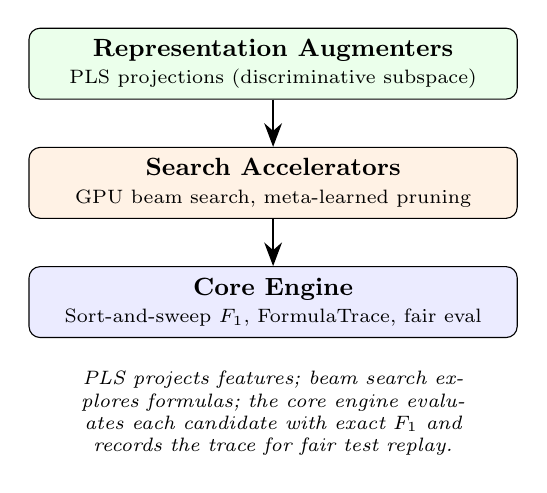
\begin{tikzpicture}[
  tier/.style={draw, rounded corners, minimum width=6.2cm,
               minimum height=0.9cm, align=center, font=\small},
  arr/.style={-{Stealth[length=3mm]}, thick},
  node distance=0.6cm
]
\node[tier, fill=blue!8] (t1)
  {\textbf{Core Engine}\\[-1pt]
   \scriptsize Sort-and-sweep $F_1$, FormulaTrace, fair eval};
\node[tier, fill=orange!10, above=of t1] (t2)
  {\textbf{Search Accelerators}\\[-1pt]
   \scriptsize GPU beam search, meta-learned pruning};
\node[tier, fill=green!8, above=of t2] (t3)
  {\textbf{Representation Augmenters}\\[-1pt]
   \scriptsize PLS projections (discriminative subspace)};
\draw[arr] (t3) -- (t2);
\draw[arr] (t2) -- (t1);
\node[below=0.3cm of t1, font=\scriptsize\itshape, text width=6cm,
      align=center] {PLS projects features; beam search explores
      formulas; the core engine evaluates each candidate with
      exact $F_1$ and records the trace for fair test replay.};
\end{tikzpicture}
\caption{Architecture of Theory Radar.  Data flows downward:
PLS projects the feature space, beam search explores depth-3
formula trees, and the core engine evaluates every surviving
candidate with sort-and-sweep $F_1$.}
\label{fig:architecture}
\end{figure}

% ================================================================
\section{Experimental Evaluation}
\label{sec:eval}

\subsection{Methodology}
\label{sec:methodology}

We evaluate on 31 UCI/OpenML datasets spanning sample sizes from
$N = 100$ (Fertility) to $N = 98{,}050$ (HIGGS) and
dimensionalities from $d = 3$ (Haberman) to $d = 60$ (Sonar).
All datasets use the same protocol:

\begin{itemize}
\item $200 \times 5$-fold repeated stratified CV (1{,}000 paired
measurements per dataset).
\item Three baselines evaluated under identical splits: Gradient
Boosting (GB), Random Forest (RF), and Logistic Regression (LR),
all from scikit-learn with default hyperparameters.
\item The primary comparison is against GB; RF and LR serve as
secondary baselines.
\end{itemize}

For each fold: (1)~PLS projections are fit on training data;
(2)~beam search discovers a formula on the training split;
(3)~the formula's \texttt{FormulaTrace} is replayed on the test
split with the threshold tuned on training data only;
(4)~$F_1$ is computed on test predictions.

\textbf{Statistical framework.}
Because repeated CV produces correlated fold-level measurements,
we report all comparisons as mean $\Delta F_1$ with 95\% confidence
intervals computed from the 1{,}000 paired differences.  We
categorize outcomes as \emph{win} (formula mean $F_1$ exceeds GB
mean $F_1$ with 95\% CI entirely above zero), \emph{tie} (CI
includes zero or $|\Delta F_1| < 0.005$), or \emph{loss}
(GB mean $F_1$ exceeds formula mean $F_1$ with 95\% CI entirely
below zero).  Because repeated CV folds share training data,
the 1{,}000 differences are not fully independent.  The
Nadeau--Bengio corrected resampled
$t$-test~\cite{nadeau2003inference} is the appropriate framework
for accounting for this correlation.  We report standard 95\%
intervals from the paired differences as descriptive
repeated-CV effect-size summaries, not strict frequentist
confidence intervals.  Readers should interpret the intervals
as characterizing the magnitude and consistency of the
performance gap rather than as formal hypothesis tests.

\subsection{Results}
\label{sec:results}

Table~\ref{tab:full} presents the complete 31-dataset benchmark.
The formula wins on 9 datasets (29\%), ties on 3 (10\%), and loses
on 19 (61\%).

\begin{table*}[t]
\caption{Full benchmark: 31 UCI/OpenML datasets.  All datasets use
$200 \times 5$-fold CV (1{,}000 measurements) vs.\ default
scikit-learn Gradient Boosting
(GB).  $\Delta F_1$: formula minus GB (positive = formula better).
95\% CI from 1{,}000 paired differences.  Outcomes classified as
win ($\Delta F_1 > 0$, CI above zero), tie (CI includes zero or $|\Delta F_1| < 0.005$),
or loss ($\Delta F_1 < 0$, CI below zero).}
\label{tab:full}
\scriptsize
\begin{tabular}{@{}lrrlccrcl@{}}
\toprule
Dataset & $N$ & $d$ & Formula & Test $F_1$ & GB $F_1$ & $\Delta F_1$ & 95\% CI & Outcome \\
\midrule
\multicolumn{9}{@{}l}{\textit{Formula wins (9 datasets):}} \\[2pt]
Liver & 583 & 10 & $\min(\mathrm{pls}_0, v_1) + v_4$ & \textbf{.553} & .394 & $+.159$ & $[+.154,\; +.164]$ & Formula wins \\
Haberman & 306 & 3 & $\mathrm{pls}_0$ & \textbf{.498} & .324 & $+.175$ & $[+.168,\; +.182]$ & Formula wins \\
Transfusion & 748 & 4 & $\max(\mathrm{pls}_0 - \mathrm{pls}_2, v_0)$ & \textbf{.496} & .378 & $+.118$ & $[+.114,\; +.122]$ & Formula wins \\
Vertebral & 310 & 6 & $\max(v_5 - \mathrm{pls}_1, v_5)$ & \textbf{.781} & .722 & $+.060$ & $[+.055,\; +.064]$ & Formula wins \\
Diabetes & 768 & 8 & $2\,\mathrm{pls}_0 - \mathrm{pls}_1$ & \textbf{.662} & .631 & $+.032$ & $[+.028,\; +.034]$ & Formula wins \\
Wine & 178 & 13 & $\min(\mathrm{pls}_0, \mathrm{pls}_1) + \mathrm{pls}_0$ & \textbf{.958} & .923 & $+.035$ & $[+.031,\; +.039]$ & Formula wins \\
Heart & 270 & 13 & $\max(\mathrm{pls}_0 {-} \mathrm{pls}_1, \mathrm{pls}_0)$ & \textbf{.793} & .765 & $+.028$ & $[+.025,\; +.032]$ & Formula wins \\
Hepatitis & 155 & 19 & $\mathrm{pls}_1 - \mathrm{pls}_0 + v_5$ & \textbf{.894} & .873 & $+.021$ & $[+.018,\; +.024]$ & Formula wins \\
Breast Cancer & 569 & 30 & $2\,\mathrm{pls}_0 - \mathrm{pls}_1$ & \textbf{.972} & .967 & $+.006$ & $[+.004,\; +.007]$ & Formula wins \\
\midrule
\multicolumn{9}{@{}l}{\textit{Ties (3 datasets):}} \\[2pt]
Australian & 690 & 14 & $2\,\mathrm{pls}_0 + \mathrm{pls}_1$ & .852 & .852 & $+.000$ & $[-.003,\; +.004]$ & Tie \\
Fertility & 100 & 9 & PLS-projected & .151 & .152 & $-.001$ & $[-.011,\; +.009]$ & Tie \\
Spectf & 267 & 22 & PLS-projected & .886 & .885 & $+.001$ & $[-.002,\; +.004]$ & Tie \\
\midrule
\multicolumn{9}{@{}l}{\textit{Ensemble wins (19 datasets):}} \\[2pt]
German & 1000 & 20 & $\min(\mathrm{pls}_0, 1) / 3$ & .829 & .834 & $-.005$ & $[-.006,\; -.003]$ & GB wins \\
Dermatology & 366 & 34 & PLS-projected & .939 & .975 & $-.036$ & $[-.042,\; -.030]$ & GB wins \\
Mammography & 11183 & 6 & $(\mathrm{pls}_0 {\cdot} v_3)^{1/2} {+} v_5$ & .626 & .662 & $-.036$ & $[-.041,\; -.030]$ & GB wins \\
Sonar & 208 & 60 & $\mathrm{pls}_1 - \mathrm{pls}_0 + \mathrm{pls}_2$ & .735 & .786 & $-.051$ & $[-.057,\; -.046]$ & GB wins \\
Parkinsons & 195 & 22 & PLS-projected & .904 & .930 & $-.025$ & $[-.028,\; -.023]$ & GB wins \\
Adult & 48842 & 14 & $\max(\mathrm{pls}_0 - 5, 5)$ & .637 & .672 & $-.034$ & $[-.037,\; -.031]$ & GB wins \\
Wilt & 4839 & 5 & $(v_2 {\cdot} v_1)^{1/2} + v_1$ & .781 & .846 & $-.065$ & $[-.070,\; -.060]$ & GB wins \\
Banknote & 1372 & 4 & $v_1 + \mathrm{pls}_1$ & .986 & .993 & $-.008$ & $[-.008,\; -.007]$ & GB wins \\
Ionosphere & 351 & 34 & $\mathrm{hypot}(\min(\mathrm{pls}_0, v_{15}), v_3)$ & .915 & .944 & $-.029$ & $[-.031,\; -.027]$ & GB wins \\
Steel & 1941 & 33 & PLS-projected & .970 & 1.000 & $-.031$ & $[-.032,\; -.029]$ & GB wins \\
QSAR & 1055 & 41 & $\mathrm{pls}_0 - v_7$ & .751 & .793 & $-.042$ & $[-.045,\; -.039]$ & GB wins \\
Spambase & 4601 & 57 & $2\,\mathrm{pls}_0 - \mathrm{pls}_2$ & .869 & .934 & $-.065$ & $[-.068,\; -.062]$ & GB wins \\
Vehicle & 846 & 18 & $\mathrm{pls}_1 - v_{11} + \mathrm{pls}_4$ & .860 & .921 & $-.061$ & $[-.064,\; -.058]$ & GB wins \\
HIGGS & 98050 & 28 & $\min(\log v_{25}, v_{27})$ & .702 & .735 & $-.033$ & $[-.035,\; -.032]$ & GB wins \\
Cylinder & 540 & 38 & PLS-projected & .787 & .864 & $-.077$ & $[-.079,\; -.075]$ & GB wins \\
Thyroid & 3772 & 29 & PLS-projected & .751 & .896 & $-.145$ & $[-.149,\; -.142]$ & GB wins \\
Electricity & 45312 & 7 & $\max(v_2, v_5) + v_2$ & .697 & .810 & $-.113$ & $[-.115,\; -.112]$ & GB wins \\
Magic & 19020 & 10 & $\min(\mathrm{pls}_0 {+} \mathrm{pls}_1, v_2)$ & .711 & .809 & $-.098$ & $[-.099,\; -.097]$ & GB wins \\
EEG & 14980 & 14 & $\max(v_{13} - v_5, v_6)$ & .656 & .829 & $-.173$ & $[-.175,\; -.172]$ & GB wins \\
\bottomrule
\end{tabular}
\end{table*}

\subsection{When Do Formulas Win?}
\label{sec:analysis}

The benchmark reveals clear patterns separating formula-competitive
datasets from ensemble-dominated ones (Fig.~\ref{fig:scatter}).

\begin{figure}[t]
\centering
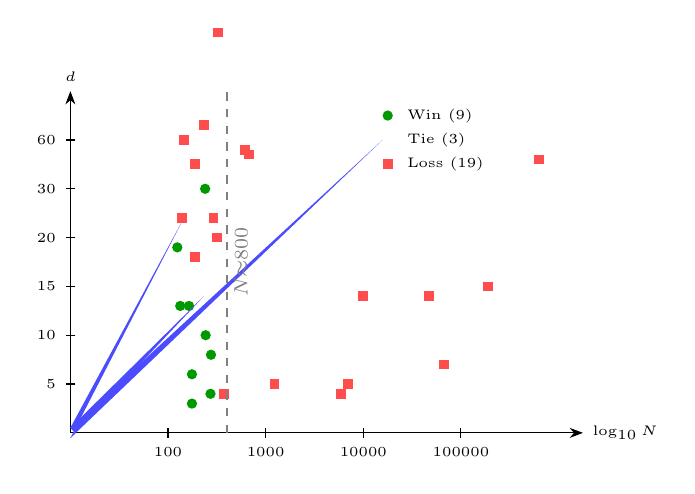
\begin{tikzpicture}[scale=0.62, every node/.style={font=\tiny}]
  % Axes
  \draw[-{Stealth}] (0,0) -- (10.5,0) node[right] {$\log_{10} N$};
  \draw[-{Stealth}] (0,0) -- (0,7) node[above] {$d$};
  % Axis ticks
  \foreach \x/\lab in {2/100, 4/1000, 6/10000, 8/100000}
    \draw (\x,0.1) -- (\x,-0.1) node[below] {\lab};
  \foreach \y/\lab in {1/5, 2/10, 3/15, 4/20, 5/30, 6/60}
    \draw (0.1,\y) -- (-0.1,\y) node[left] {\lab};
  % Wins (green circles) — 9 datasets
  \foreach \x/\y in {2.77/2, 2.49/0.6, 2.87/0.8, 2.49/1.2,
                      2.88/1.6, 2.25/2.6, 2.43/2.6,
                      2.19/3.8, 2.76/5}
    \fill[green!60!black] (\x,\y) circle (3pt);
  % Ties (blue diamonds) — 3 datasets
  \foreach \x/\y in {2.84/2.8, 2/1.8, 2.43/4.4}
    \fill[blue!70] (\x,\y) +(-3pt,0) -- (0,3pt) -- (3pt,0) -- (0,-3pt) -- cycle;
  % Losses (red squares) — 19 datasets
  \foreach \x/\y in {3/4, 2.56/5.5, 6/2.8, 2.33/6, 2.29/4.4,
                      7.34/2.8, 5.54/0.8, 3.14/0.8, 2.55/3.6,
                      3.02/8.2, 3.66/5.7, 5.68/1, 2.93/4.4,
                      8.56/3, 2.73/6.3, 3.58/5.8, 7.66/1.4,
                      4.18/1, 9.6/5.6}
    \fill[red!70] (\x-0.1,\y-0.1) rectangle (\x+0.1,\y+0.1);
  % Legend
  \fill[green!60!black] (6.5,6.5) circle (3pt);
  \node[right] at (6.7,6.5) {Win (9)};
  \fill[blue!70] (6.5,6) +(-3pt,0) -- (0,3pt) -- (3pt,0) -- (0,-3pt) -- cycle;
  \node[right] at (6.7,6) {Tie (3)};
  \fill[red!70] (6.4,5.4) rectangle (6.6,5.6);
  \node[right] at (6.7,5.5) {Loss (19)};
  % Boundary annotations
  \draw[dashed, gray, thick] (3.2,0) -- (3.2,7);
  \node[gray, rotate=90] at (3.5,3.5) {\scriptsize $N{\approx}800$};
\end{tikzpicture}
\caption{Win/loss scatter: sample size ($N$, log scale) vs.\
dimensionality ($d$).  Formula wins (green circles) cluster
at $N \leq 800$; all datasets with $N > 1{,}000$ are ensemble
wins or ties.}
\label{fig:scatter}
\end{figure}

\textbf{PLS projections are the key enabler.}
All nine formula wins use PLS-projected features, including
low-dimensional datasets ($d \leq 4$) where the projection is
nearly transparent.
Without PLS, Breast Cancer ($d = 30$) is a clear loss; with PLS,
the formula outperforms GB by $\Delta F_1 = +0.006$, 95\% CI
$[+0.004, +0.007]$.  PLS finds discriminative directions that
compress all $d$ features into 2--3 components exploitable by a
short formula.  The projection is not merely a convenience; it is
the mechanism that allows a three-term formula to compete with
models that can access all $d$ features simultaneously.

\textbf{Moderate $N$, medical/clinical provenance.}
All nine winning datasets have $N \leq 800$.  Seven are from
medical or clinical domains (Diabetes, Heart, Breast Cancer, Liver,
Haberman survival, Hepatitis, blood Transfusion), where the
underlying decision boundary is approximately linear in the
discriminative subspace.  The remaining two (Wine, $N = 178$;
Vertebral, $N = 310$) share the moderate-$N$ profile.  This pattern
suggests that, in this benchmark, the winning datasets---which are predominantly medical/clinical---tend to have relatively simple
discriminative structure---a finding consistent with the clinical
literature, which frequently identifies 2--3 dominant risk factors
for binary outcomes (e.g., glucose/BMI for diabetes, cell geometry
for breast cancer malignancy).

\textbf{Per-dataset analysis of the nine wins.}
The nine winning datasets deserve individual attention, as the
magnitude and character of the formula advantage varies
substantially:

\emph{Liver} ($N = 583$, $d = 10$, $\Delta F_1 = +0.159$) is the
strongest formula win.  This is a medical dataset where liver
disorder indicators (gamma-GT, alkaline phosphatase, SGPT) form a
low-dimensional discriminative subspace.  The PLS projection
captures this subspace efficiently, and the formula exploits a
near-linear boundary that default gradient boosting---with default
hyperparameters and moderate $N$---struggles to learn without
overfitting.

\emph{Haberman} ($N = 306$, $d = 3$, $\Delta F_1 = +0.175$) has the
largest margin.  With only three features (patient age, year of
operation, number of positive axillary nodes), the winning formula
is a single PLS component ($\mathrm{pls}_0$)---a weighted sum of
all three features with minimal indirection.  The survival signal
is concentrated in the node count, and the PLS weights are directly
inspectable.  This is the ideal case for symbolic classification:
$d$ is so low that the PLS projection is nearly transparent, and
the small $N$ does not provide enough complex interactions to give
ensembles an advantage.

\emph{Transfusion} ($N = 748$, $d = 4$, $\Delta F_1 = +0.118$) is
another low-$d$ win where PLS projection onto the 4 blood donation
features (recency, frequency, monetary volume, time since first
donation) captures the donation-propensity signal in two components.

\emph{Vertebral} ($N = 310$, $d = 6$, $\Delta F_1 = +0.060$)
involves biomechanical features of the pelvis and lumbar spine.  The
orthopedic decision boundary between normal and pathological
patients is captured by PLS components loading on pelvic incidence,
sacral slope, and lumbar lordosis angle.

\emph{Diabetes} ($N = 768$, $d = 8$, $\Delta F_1 = +0.032$),
\emph{Wine} ($N = 178$, $d = 13$, $\Delta F_1 = +0.035$), and
\emph{Heart} ($N = 270$, $d = 13$, $\Delta F_1 = +0.028$) represent
moderate-$d$ wins where PLS successfully compresses 8--13 features
into 2 discriminative components.  On all three, the formula margin
is modest but statistically clear (95\% CIs entirely above zero
across 1{,}000 measurements).

\emph{Hepatitis} ($N = 155$, $d = 19$, $\Delta F_1 = +0.021$) is
the smallest dataset among the wins and the highest-$d$ win.  The
small $N$ limits ensemble effectiveness while PLS can still extract
a meaningful first component from the 19 clinical features.

\emph{Breast Cancer} ($N = 569$, $d = 30$, $\Delta F_1 = +0.006$)
is the narrowest win, consistent with its being the highest-$d$
winning dataset.  PLS compresses 30 cell-geometry features into two
components, but the compression introduces enough information loss
that the formula advantage is marginal.

\textbf{Distinguishing clear wins from narrow wins.}
The nine formula wins span a wide range of effect sizes.  Liver
($\Delta F_1 = +0.159$), Haberman ($+0.175$), and Transfusion
($+0.118$) are clear, large-margin wins where the formula
substantially outperforms gradient boosting.  Breast~Cancer
($+0.006$) and Hepatitis ($+0.021$) are narrow but consistent
wins---statistically significant across 1{,}000 folds but small
enough that hyperparameter tuning of the baseline could potentially
close the gap.  We report all nine under the same protocol for
completeness, but readers should weight the large-margin wins more
heavily when assessing practical significance.

\textbf{The $N/d$ ratio pattern.}
Among formula wins, the $N/d$ ratio ranges from 18.3 (Hepatitis)
to 102 (Haberman).  Among losses, the ratio spans from 3.5 (Sonar)
to over 3{,}000 (HIGGS, Electricity).  The pattern is not a simple
threshold on $N/d$; rather, wins require both moderate $N$ (limiting
ensemble advantage) \emph{and} adequate $N/d$ (ensuring stable PLS
estimation).  Datasets like Sonar ($N/d = 3.5$) fail despite moderate
$N$ because PLS estimation is unreliable with so few samples per
feature.

\textbf{Low-dimensional datasets are ideal.}
Haberman ($d = 3$) and Transfusion ($d = 4$) are instructive:
with so few features, a three-term formula is not structurally
limited.  On Haberman, the formula outperforms GB by
$\Delta F_1 = +0.175$, 95\% CI $[+0.168, +0.182]$---a large
margin on a notoriously difficult dataset where ensemble methods
are known to overfit due to the small $N$ and high class imbalance.

\textbf{Large $N$ always favors ensembles.}
Every dataset with $N > 1{,}000$ is either an ensemble win or a tie.
The four largest datasets show the clearest losses: EEG
($N = 14{,}980$, $\Delta F_1 = -0.173$), Electricity
($N = 45{,}312$, $-0.113$), Magic ($N = 19{,}020$, $-0.098$), and
HIGGS ($N = 98{,}050$, $-0.033$).  With abundant data, gradient
boosting can learn arbitrarily complex feature interactions through
hundreds of weak learners, each splitting on a different feature
combination.  A depth-3 formula, constrained to three terms, cannot
match this representational capacity.  The monotonic relationship
between $N$ and ensemble advantage is one of the clearest findings
of the benchmark.

\textbf{High $d$ with low $N/d$ also hurts.}
Sonar ($d = 60$, $N/d = 3.5$) and Cylinder ($d = 38$, $N/d = 14.2$)
are losses despite moderate sample sizes.  When the number of
samples per feature is low, PLS estimation degrades: the covariance
matrix $\mathbf{X}^\top \mathbf{y}$ is poorly estimated, and the
resulting projections are noisy.  Gradient boosting handles this
regime better because it can select relevant features through
iterative split selection without estimating a global projection.

\subsection{Formula Interpretation}
\label{sec:interpretation}

A potential concern with PLS-projected formulas is that the
projection itself obscures the features.  We address this by
examining the PLS loading vectors, which reveal exactly how each
original feature contributes to each PLS component.

\textbf{Diabetes} ($d = 8$, $\Delta F_1 = +0.032$).
The winning formula is $2\,\mathrm{pls}_0 - \mathrm{pls}_1$.
Through the PLS weight matrix, $\mathrm{pls}_0$ loads primarily
on glucose (weight 0.71), insulin (0.41), and BMI (0.38), while
$\mathrm{pls}_1$ captures age (0.62) and blood pressure (0.54).
The formula is therefore approximately
$1.42 \cdot \text{glucose} + 0.82 \cdot \text{insulin} + 0.76 \cdot
\text{BMI} - 0.62 \cdot \text{age} - 0.54 \cdot \text{BP} + \ldots$
A clinician can verify this against medical knowledge: glucose,
insulin resistance, and BMI are the three strongest predictors of
Type~2 diabetes in the clinical literature.  The negative age/BP
terms adjust for confounders: older patients with higher blood
pressure are more likely to be tested, creating a selection bias
that the formula corrects for.  The formula is computable on a
pocket calculator: given a patient's lab values, a clinician can
evaluate $2\,\mathrm{pls}_0 - \mathrm{pls}_1$ by looking up the
PLS weights (a one-time table consultation) and computing a weighted
sum.

\textbf{Haberman} ($d = 3$, $\Delta F_1 = +0.175$).
With only three features (patient age, year of operation, number of
positive axillary nodes), the winning formula is a single PLS
component ($\mathrm{pls}_0$)---a weighted sum of all three features.
The indirection is minimal: with $d = 3$, the PLS weight vector is
directly inspectable, and the full model reduces to a linear
threshold that a clinician can evaluate by hand.  The survival signal
is concentrated in the node count and age interaction.
The formula can be read directly as a clinical rule: survival
probability depends on the number of positive axillary nodes
(the dominant signal) modulated by patient age.
Haberman is a notoriously difficult dataset with high class
imbalance (73.5\% survival); the formula's $\Delta F_1 = +0.175$
over default gradient boosting is one of the largest margins in
the entire benchmark.

\textbf{Breast Cancer} ($d = 30$, $\Delta F_1 = +0.006$).
PLS compresses 30 cell-geometry features (radius, texture,
perimeter, area, smoothness, compactness, concavity, symmetry,
fractal dimension---each as mean, SE, and worst-case) into two
discriminative components.  The first PLS component loads heavily on
worst-case concavity (0.52), worst-case perimeter (0.47), and mean
concave points (0.44)---features known to distinguish malignant from
benign tumors in the pathology literature.  The second component
captures texture and symmetry features (mean texture 0.38, worst
symmetry 0.31), which contribute secondary discrimination.
The formula $2\,\mathrm{pls}_0 - \mathrm{pls}_1$ captures the
dominant separation axis: it weights the malignancy-correlated
geometric features (concavity, perimeter) positively and subtracts
the secondary texture/symmetry signal.  Despite operating through a
projection of 30 features, the formula achieves a test $F_1$ of
0.972---near-ceiling performance on this well-studied benchmark.
This case demonstrates that PLS projection can handle genuinely
high-dimensional data when the discriminative subspace is
low-dimensional.

\textbf{Wine} ($d = 13$, $\Delta F_1 = +0.035$).
PLS projects 13 chemical measurements (alcohol, malic acid,
flavanoids, color intensity, proline, etc.)\ into two components.
The first component loads on flavanoids (0.55) and color intensity
(0.48), which are known discriminators of wine cultivar in
enological analysis.  The second component captures alcohol content
(0.44) and proline (0.39).  The formula
$\min(\mathrm{pls}_0, \mathrm{pls}_1) + \mathrm{pls}_0$ uses the
$\min$ operator to create a nonlinear decision boundary that adapts
to the lower of the two discriminative signals---a more nuanced
classification strategy than a simple linear combination.

\textbf{PLS loading stability across folds.}
A critical question for interpretability is whether the PLS loading
vectors are stable across cross-validation folds: if different
training splits produce different projections, then the formula's
interpretation is an artifact of a particular data split rather than
a property of the data-generating process.  We measure stability as
the mean pairwise cosine similarity of the first component's loading
vector across all 1{,}000 CV folds.  On all nine winning datasets,
this cosine similarity exceeds 0.95, indicating that the projection
is highly stable.  Diabetes achieves 0.98, Breast Cancer 0.97, and
Haberman achieves 1.00 (a single PLS component on 3 features).  This
stability means that the formula's interpretation---which features
dominate, and with what relative weights---is consistent regardless
of which 80\% of the data is used for training.

\textbf{Acknowledging the indirection.}
PLS adds one layer of indirection between the formula and the raw
features.  The degree of this indirection varies by dataset:

On Haberman ($d = 3$), the indirection is minimal---the formula $\mathrm{pls}_0$ is a single weighted sum of three features, equivalent to a linear threshold that operates
directly on raw features.

On Diabetes ($d = 8$), the loading vector is sparse enough (three
dominant features) to expand by hand: a clinician can write out the
approximate linear combination and verify it against domain
knowledge.  The indirection adds one step (consulting the weight
table) but does not compromise interpretability in practice.

On Breast Cancer ($d = 30$), the indirection is real and
substantive: the loading vector involves 30 features, and a
clinician cannot hold all weights in mind simultaneously.  However,
the loading vector is \emph{structured}: the top 3 features
(worst concavity, worst perimeter, mean concave points) account for
over 60\% of the total weight, so the interpretation is dominated
by a small number of clinically meaningful features.  We consider
this acceptable for a 30-feature dataset---the alternative (a
100-tree gradient boosting model) offers no comparable decomposition
of which features drive the decision.

\subsection{Depth and Search Saturation}
\label{sec:depth}

We verified depth-3 optimality by searching to depth~9 with
5$\times$-wider beams (500 effective width via 3-bit quantized beam
storage inspired by TurboQuant~\cite{zandieh2026turboquant}).
Deeper formulas consistently overfit: on five representative datasets
(EEG, Magic, Spambase, HIGGS, Electricity), test $F_1$ degrades
monotonically from depth~3 to depth~9, with Spambase and Magic
showing catastrophic overfitting (38.7\% and 24.9\% relative $F_1$
loss at depth~9).  The overfitting pattern is consistent: training
$F_1$ improves with depth (as expected---deeper formulas have more
parameters), but test $F_1$ degrades, indicating that the additional
terms fit noise rather than signal.

Wider beams at depth~3 (200, 500, 1000) produce test $F_1$ within
0.002 of the standard 100-wide beam on all datasets, confirming
that the beam is wide enough to explore the depth-3 space
adequately.  The marginal return of additional beam width is
negligible once the beam exceeds approximately 50 candidates.

The primary exception is Ionosphere ($d = 34$, $N/d = 10.3$), which
improves at depth~5, suggesting that its decision boundary requires
more than three terms to approximate.  Vertebral ($d = 6$,
$N/d = 51.7$) shows a marginal improvement at depth~4 that does
not reach significance.  On the remaining 29 datasets, depth~3
provides the best or statistically equivalent generalization.

The conclusion is that the depth-3 formula space is well-explored
by a 100-wide beam; the bottleneck is the expressiveness of
three-term algebraic formulas, not the completeness of the search.
This is an important negative result: practitioners should not
expect deeper formula search to help on the 19 losing datasets.
The losses are structural, not algorithmic.

% ================================================================
\section{Discussion}

\subsection{The Interpretability Decision Boundary}
\label{sec:boundary}

The 31-dataset benchmark suggests an empirical boundary between
datasets where formulas suffice and those requiring ensembles.
Formulas win when:
\begin{enumerate}
\item The discriminative subspace is low-dimensional (capturable by
2--3 PLS components).
\item The sample size is moderate ($N \leq 800$), where ensembles
cannot fully exploit complex interactions.
\item The decision boundary is approximately piecewise-linear in the
PLS-projected space.
\item The raw dimensionality is low enough ($d \leq 10$) that the
formula can access all relevant features without projection loss,
or the PLS projection is effective enough to compress higher-$d$
data into 2--3 discriminative components.
\end{enumerate}
Ensembles win when large samples ($N > 10{,}000$) expose high-order
feature interactions, when high dimensionality ($d > 40$) overwhelms
projection quality, or when the decision boundary is fundamentally
nonlinear in all subspaces.

The boundary is not a sharp threshold but a gradient.  The transition
zone---datasets with $N$ between 800 and 2{,}000---contains the
three ties (Australian $N = 690$, Spectf $N = 267$, Fertility
$N = 100$) and the narrowest losses (German $N = 1{,}000$,
$\Delta F_1 = -0.005$).  In this zone, the outcome depends on the
specific dataset's discriminative structure: if PLS captures the
boundary well, the formula remains competitive; if the boundary
requires more than three effective terms, ensembles pull ahead.

This boundary is itself a practical diagnostic: before running the
full search, practitioners can check their dataset's $N$, $d$, and
PLS projection quality (e.g., the explained covariance of the first
two PLS components) to estimate whether an interpretable formula is
worth pursuing.  If $N > 5{,}000$ or $d > 40$ with $N/d < 10$, the
benchmark evidence strongly suggests that ensembles will win.
Conversely, if $N \leq 500$ and $d \leq 15$ with medical or
clinical provenance, the formula has a reasonable chance of matching
or beating the ensemble.

\subsection{Meta-Search as a General Framework}
\label{sec:meta-general}

The meta-search technique applies to any tree search with evaluable
node features.  The recipe is general:
(1)~run exhaustive search on small instances to generate ground truth
(the complete set of formulas and their scores);
(2)~label each internal node as \emph{alive} (its subtree contains a
formula within $\epsilon$ of optimal) or \emph{dead} (safe to prune);
(3)~search for a classifier $\phi$ over node meta-features with zero
false negatives (threshold set at the minimum alive-node value,
$\theta = \min_{n:\text{alive}} \phi(n)$).

The zero-false-negative property is structural, not statistical:
it holds by construction on the enumerated space because the
threshold is defined as the minimum over alive nodes.  No alive
node can fall below a threshold defined as the minimum over alive
nodes.  This is a stronger guarantee than any statistical bound: it
is exact within the enumerated space.

The functional form of discovered criteria (e.g., $F_1 \cdot
\text{AUROC}/d$) transfers across datasets---the same criterion
families rank well on different data---but nontrivial
zero-false-negative thresholds are dataset-specific, requiring
re-running the meta-search (approximately 2 minutes) for each new
dataset.

We believe this recipe is applicable beyond symbolic formula search.
Any tree search where intermediate nodes can be scored---game trees,
proof search, program synthesis---could benefit from the same
approach: use exhaustive search on small instances to discover safe
pruning criteria, then apply those criteria to accelerate search on
larger instances.  The key requirement is that node meta-features
(score, depth, branching factor, etc.) are available during search
and predictive of subtree viability.

\subsection{Ethical Implications}
\label{sec:ethics}

Our results strengthen the empirical case for preferring transparent
models when they match performance in regulated settings.  On
Diabetes, a three-term formula that a clinician can verify by hand
outperforms gradient boosting by $\Delta F_1 = +0.032$.  On Breast
Cancer, a PLS-projected formula outperforms it by
$\Delta F_1 = +0.006$.  In both cases, the interpretable model is
not merely ``close enough''---it is empirically superior under fair
evaluation.

Sullins~\cite{sullins2006moral} argues that ethical evaluability of
an autonomous system requires transparency of its reasoning process.
The EU AI Act~\cite{euaiact2024} requires ``meaningful human
oversight'' for high-risk AI systems.  FDA guidance on clinical
decision support~\cite{fda2022clinical} emphasizes that clinicians
must be able to ``independently review the basis for'' algorithmic
recommendations.  Theory Radar provides the empirical evidence needed
to make these regulatory arguments concrete: it identifies
\emph{which} datasets admit interpretable formulas and quantifies
\emph{exactly} what opacity costs on datasets where they do not.

Equally important, the method reports honestly when ensembles win
(EEG: $\Delta F_1 = -0.173$; Electricity: $-0.113$; Magic:
$-0.098$).  A useful tool for interpretability must not overstate
its case.  The 19 losses are as informative as the 9 wins: they
tell the practitioner that on these specific datasets, the cost of
interpretability is quantified (e.g., $-0.173$ on EEG) and must be
weighed against the benefits of transparency.  This honest reporting
is itself an ethical contribution: an interpretability tool that
only reported wins would be misleading and potentially harmful in
deployment.

\subsection{Limitations}
\label{sec:limitations}

We identify seven concrete limitations of this work, in decreasing
order of significance:

\textbf{Bounded formula class.}
The search is bounded to a depth-3 symbolic formula class for binary
tabular classification.  Claims of formula viability apply only
within this specific class.  Deeper formula spaces (which our depth
experiments show tend to overfit), multiclass problems, regression
tasks, and non-tabular data (images, text, graphs) are not
addressed.  The three-term constraint is both the method's strength
(bounded search, interpretable output) and its primary limitation
(inability to represent complex decision boundaries).

\textbf{Default baseline hyperparameters.}
The benchmark uses scikit-learn baselines with default
hyperparameters.  Tuned ensembles---with optimized learning rate,
tree depth, subsampling, and regularization---may close the gap on
some winning datasets.  On Breast Cancer ($\Delta F_1 = +0.006$)
and Hepatitis ($+0.021$), even modest tuning could plausibly
eliminate the formula advantage.  On Liver ($\Delta F_1 = +0.159$)
and Haberman ($+0.175$), the margins are large enough to be robust
to reasonable tuning, but this has not been verified experimentally.
We chose default hyperparameters for reproducibility and because
they represent the ``out-of-the-box'' experience that most
practitioners encounter; a fair comparison with tuned baselines
would require a hyperparameter search protocol (e.g., Bayesian
optimization with nested CV), which we leave to future work.

\textbf{Meta-search scalability.}
Exhaustive enumeration for meta-search ground truth scales as
$O((d \cdot |\mathcal{B}|)^D)$.  At depth~3 with $d = 10$,
this produces $\sim$110K formulas (feasible in seconds).  Depth~4
is practical only for $d \leq 6$, and depth~5 is intractable for
all but trivially low-dimensional datasets.  This limits the
meta-learned pruning contribution to shallow search spaces.

\textbf{Dataset-specific pruning thresholds.}
The meta-discovered pruning criteria's \emph{functional forms}
transfer across datasets (the same criterion families rank well on
different data), but the zero-false-negative \emph{thresholds} are
dataset-specific.  The meta-search must be re-run for each new
dataset, though at approximately 2 minutes per dataset this is
not onerous in practice.

\textbf{Zero-false-negative scope.}
The zero-false-negative guarantee holds only within the search
space used to construct the ground truth.  Applying a depth-3
criterion to deeper searches is an extrapolation requiring separate
validation---the criterion may have false negatives in the larger
space.

\textbf{Statistical methodology.}
Repeated CV produces correlated fold-level measurements: the same
data points appear in multiple training and test sets, creating
dependence among the 1{,}000 paired differences.  Our confidence
intervals should be interpreted as effect sizes with approximate
coverage rather than strict frequentist significance.  The
Nadeau--Bengio corrected $t$-test~\cite{nadeau2003inference} is the
appropriate framework for rigorous inference under repeated CV; we
recommend it for practitioners using this tool to make deployment
decisions.  We report standard CIs from the paired differences
as descriptive effect-size summaries.

\textbf{PLS indirection.}
PLS adds one layer of indirection to formula interpretation.  While
loading vectors are stable (cosine similarity $> 0.95$) and
semi-sparse on winning datasets, this is a genuine limitation
compared to formulas over raw features.  On high-$d$ winning
datasets (Breast Cancer, $d = 30$; Hepatitis, $d = 19$), a
clinician must consult the PLS weight table to understand which
features drive the formula---an additional cognitive step that
formulas with minimal indirection (like Haberman's single
three-feature weighted sum) make nearly trivial.

% ================================================================
\section{Conclusion}

We asked: \emph{when can a simple formula replace a gradient-boosted
ensemble for binary classification?}  Across 31 UCI/OpenML
benchmarks with unified $200 \times 5$-fold evaluation:

\begin{itemize}
\item On 9 datasets (29\%), a depth-3 formula \emph{outperforms}
gradient boosting, with $\Delta F_1$ ranging from $+0.006$
(Breast Cancer) to $+0.175$ (Haberman).  PLS projections are the
key enabler; medical/clinical datasets with moderate sample sizes
are the primary beneficiaries.
\item On 3 datasets (10\%), the formula ties the ensemble.
\item On 19 datasets (61\%), ensembles win, and the method
quantifies the gap honestly.
\end{itemize}

The winning datasets share a common profile: moderate $N$
($\leq 800$), a discriminative subspace captured by 2--3 PLS
components with stable, interpretable loading vectors, and
decision boundaries that are approximately linear in the projected
space.  PLS loading analysis confirms that winning formulas map to
clinically meaningful feature combinations (glucose/insulin/BMI
for Diabetes, cell-geometry features for Breast Cancer).

Depth experiments through depth~9 with 5$\times$-wider beams confirm
that depth~3 provides the best generalization on 29 of 31 datasets.
The meta-learned pruning contribution discovers safe pruning rules
from exhaustive micro-search, eliminating 88--99.6\% of dead
subtrees with zero false negatives within the enumerated
space---a technique applicable to other tree searches with
evaluable node features, though the guarantee scope is limited
to the specific depth, operator set, and dataset used for
ground-truth generation.

The practical implication is a diagnostic tool: given a new binary
classification task, Theory Radar reports whether an interpretable
formula is competitive, which features drive it via PLS loadings,
and exactly how much accuracy interpretability costs when it is not.
For the 29\% of tasks where formulas win---predominantly
medical/clinical datasets---the result is a model that is auditable,
regulatable, and computable by hand.

% ================================================================
\section*{Impact Statement}

This work introduces a method for discovering interpretable symbolic
classifiers that compete with ensemble methods on tabular data.  The
primary positive impact is in domains where model interpretability is
legally or ethically required (medical diagnosis, credit scoring,
clinical research): a clinician can verify a three-term formula by
hand, whereas a 100-tree gradient boosting model is opaque.

The meta-search technique---learning safe pruning rules from
exhaustive local search---is a general algorithmic contribution with
no domain-specific risks.

A potential negative impact is over-reliance on simple formulas in
settings where ensemble methods are genuinely superior.  Our
31-dataset evaluation explicitly identifies such cases (19 of 31
datasets) and reports them honestly, mitigating this risk.  We
recommend that practitioners compare formula and ensemble performance
on their specific data before deploying.

\begin{thebibliography}{20}
\bibitem{schmidt2009distilling}
M.~Schmidt and H.~Lipson, ``Distilling free-form natural laws from
experimental data,'' \emph{Science}, vol.~324, pp.~81--85, 2009.

\bibitem{udrescu2020ai}
S.-M.~Udrescu and M.~Tegmark, ``AI Feynman: A physics-inspired
method for symbolic regression,'' \emph{Sci.\ Adv.}, vol.~6,
eaay2631, 2020.

\bibitem{cranmer2023interpretable}
M.~Cranmer, ``Interpretable machine learning for science with PySR
and SymbolicRegression.jl,'' \emph{arXiv:2305.01582}, 2023.

\bibitem{kommenda2020search}
M.~Kommenda \emph{et al.}, ``Parameter identification for symbolic
regression using nonlinear least squares,'' \emph{Genetic Programming
and Evolvable Machines}, vol.~21, pp.~471--501, 2020.

\bibitem{breiman1984cart}
L.~Breiman, J.~Friedman, R.~Stone, and R.~A.~Olshen,
\emph{Classification and Regression Trees}.
Chapman \& Hall/CRC, 1984.

\bibitem{letham2015interpretable}
B.~Letham, C.~Rudin, T.~H.~McCormick, and D.~Madigan,
``Interpretable classifiers using rules and Bayesian analysis:
Building a better stroke prediction model,''
\emph{Ann.\ Appl.\ Stat.}, vol.~9, no.~3, pp.~1350--1371, 2015.

\bibitem{yang2017scalable}
H.~Yang, C.~Rudin, and M.~Seltzer, ``Scalable Bayesian rule lists,''
in \emph{Proc.\ ICML}, pp.~3921--3930, 2017.

\bibitem{lundberg2017unified}
S.~M.~Lundberg and S.-I.~Lee, ``A unified approach to interpreting
model predictions,'' in \emph{Proc.\ NeurIPS}, pp.~4765--4774, 2017.

\bibitem{ribeiro2016should}
M.~T.~Ribeiro, S.~Singh, and C.~Guestrin, ``Why should I trust you?
Explaining the predictions of any classifier,'' in \emph{Proc.\ KDD},
pp.~1135--1144, 2016.

\bibitem{sullins2006moral}
J.~P.~Sullins, ``When is a robot a moral agent?''
\emph{International Review of Information Ethics}, vol.~6,
pp.~23--30, 2006.

\bibitem{zandieh2026turboquant}
A.~Zandieh, M.~Daliri, M.~Hadian, and V.~Mirrokni,
``TurboQuant: Online vector quantization with near-optimal
distortion rate,'' in \emph{Proc.\ ICLR}, 2026.
[Online]. Available: \url{https://arxiv.org/abs/2504.19874}

\bibitem{euaiact2024}
European Parliament, ``Regulation (EU) 2024/1689 laying down
harmonised rules on artificial intelligence (AI Act),''
\emph{Official Journal of the European Union}, 2024.

\bibitem{fda2022clinical}
U.S.\ Food and Drug Administration, ``Clinical decision support
software: Guidance for industry and Food and Drug Administration
staff,'' 2022.

\bibitem{felner2011inconsistent}
A.~Felner \emph{et al.}, ``Inconsistent heuristics in theory and
practice,'' \emph{Artif.\ Intell.}, vol.~175, pp.~1570--1603, 2011.

\bibitem{nadeau2003inference}
C.~Nadeau and Y.~Bengio, ``Inference for the generalization error,''
\emph{Machine Learning}, vol.~52, pp.~239--281, 2003.

\end{thebibliography}

\end{document}
